% !Mode::"TeX:UTF-8"
\documentclass[UTF8]{article}   %this [UTF8] is very important
\usepackage{ctex}               %中文支持
\usepackage{fancyhdr}           %页眉页脚
\usepackage{geometry}           %调整页边距
\geometry{a4paper,left=2cm,right=2cm}
\usepackage{underscore}         %支持下划线作为文本输入
\usepackage{graphicx}           %支持图片插入
\usepackage{float}
\usepackage{amssymb}            %支持数学符号
\usepackage{xlop}               %支持竖式除法的排版
\usepackage{booktabs}           %支持表格的线
\usepackage{caption}            %设置字体
\usepackage{listings}           %支持代码
\usepackage{varwidth}           %支持图片顶部对齐
\usepackage{amsmath}            %支持多行公式的数学环境
\usepackage{epstopdf}           %支持pdfLatex下用eps
\usepackage{multirow}           %支持合并单元格
\usepackage{longtable}          %支持长表格
\usepackage{appendix}
\usepackage{colortbl}           %支持彩色表格
\usepackage{color}
\usepackage{hyperref}
\usepackage{verbatim}			%支持代码环境
\numberwithin{equation}{section} %公式按照章节编号
\usepackage{chngcntr}			 %图片按照章节编号
\counterwithin{figure}{section}	 %图片按照章节编号

\usepackage{palatino}
\usepackage{tikz}
\usetikzlibrary{shapes.geometric, arrows}

\hypersetup{
    colorlinks=true,
    linkcolor=blue,
    filecolor=blue,      
    urlcolor=blue,
    citecolor=cyan,
}


\chead{\thesection}
\cfoot{\thepage}
\author{朱德森}
\title{MATLAB静默安装方法总结}
\begin{document}
\songti
\linespread{1.3}
\maketitle
\tableofcontents
\newpage
\section{总体流程}
\label{Sec 总体流程}

\subsection{目的}
\label{SubSec 目的}
由于 Linux 服务器一般不能上网且没有图形界面,
因此网上基于图形的教程一般不能适用于服务器安装 MATLAB 的情况。
而采用静默方式(slient)不需要调用图形界面,
可以直接通过命令行的方式进行 MATLAB 的安装。

仓库中的 PDF 描述了详细的方法,
而在该 Markdown 中只做简要的叙述。

\subsection{安装方法一}
\label{SubSec 安装方法一}
采用静默(Silent)安装的方法,
不需要图形界面。
\begin{itemize}
	\item 准备 MATLAB 镜像文件( iso 文件)
	\item 获取许可证和序列号
	\item 加载 iso 文件、配置安装文件
	\item 静默安装
	\item 激活
\end{itemize}


\subsection{安装方法二}
\label{SubSec 安装方法二}
这个方法还是需要用到图形界面,
写在这里主要作为补充。
\begin{itemize}
	\item 在 Linux 主机控制 Linux 服务器时,
	  通过 ssh 命令进行控制,
	  添加 -X 参数的情况下可以开启图形界面
	\item 通过 ./install 命令可以启动图形化的安装程序
	\item 如果没有网络,可以通过 apt-get install firefox 安装火狐浏览器,
	  然后通过命令行调用 firefox 打开浏览器进行上网认证,
	  由于 ssh 控制时已经添加了 -X 参数,
	  因此可以打开图形化的火狐浏览器
	\item 按照跟 Windows 相同的步骤进行安装激活即可
\end{itemize}

\section{具体安装方法一}
\label{Sec 具体安装方法一}
\subsection{安装示例}
\label{SubSec 安装示例}
下面将结合第{\ref{Sec MATLAB客服给的方法}}章中
客服给的安装方法进行一个实际操作的示范。
\begin{enumerate}
	\item 准备 MATLAB 镜像文件( iso 文件)

		为了下载完整版本的 MATLAB,
		以免安装的时候还需联网下载其他组件,
		iso 文件是从学校的软件正版化下载的:

		\href{https://nic.seu.edu.cn/fwzn/rjzbh1/azxkxy/MATLABazxkxy.htm}{https://nic.seu.edu.cn/fwzn/rjzbh1/azxkxy/MATLABazxkxy.htm}
	\item 获取许可证和序列号

		一般的安装流程需要通过联网登录MATLAB账号以获取激活信息,
		但是对于离线的服务器来说,
		既没有图形界面也没有网络。
		因此需要提前获取许可证和序列号。

		\begin{enumerate}
		\item 获取服务器的Host ID:
			
			客服给的教程是在终端中使用:
			
			\begin{verbatim}
			    $ /sbin/ifconfig eth0
			\end{verbatim}

			但是在我使用的服务器上并没有 eth0 ,
			这时可以直接采用 ifconfig 进行查询:
			\begin{verbatim}
			    $ ifconfig
			\end{verbatim}

			可以看到结果如图{\ref{Fig ifconfig结果}}所示:
			\begin{figure}[H]
			  \centering
			  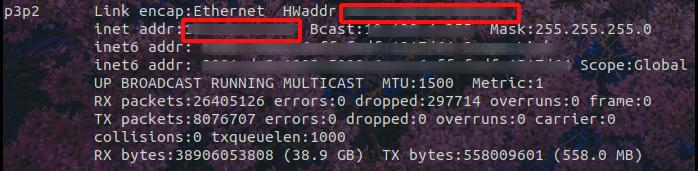
\includegraphics[width=0.7\textwidth]{./pic/ifconfig}
			  \captionsetup{font={small}}
			  \caption{ifconfig结果}
			  \label{Fig ifconfig结果}
			\end{figure}

			需要注意到 inet addr 右边的红框中所显示的 IP 地址是控制服务器所用的IP地址,
			则 HWaddr 右边红框中的序列去掉冒号即为需要用到的Host ID。

		\item 获取许可证和序列号
			
			首先需要获得服务器上登录用户名,
			在服务器上使用 whoami 命令即可。

			\begin{verbatim}
			    $ whoami
			\end{verbatim}

			通过下面的网址去获取许可证和序列号:

			\href{https://www.mathworks.com/licensecenter}{https://www.mathworks.com/licensecenter}
			
			登录MATLAB账号后,
			可以看到自己的所有许可证,
			如图{\ref{Fig 获取许可证步骤一}}所示:
			\begin{figure}[H]
			  \centering
			  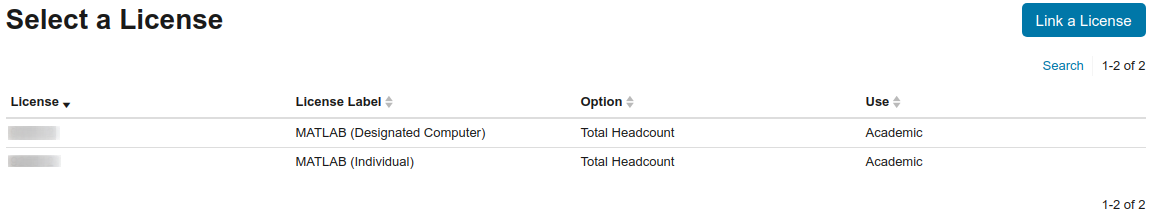
\includegraphics[width=0.7\textwidth]{./pic/license1}
			  \captionsetup{font={small}}
			  \caption{获取许可证步骤一}
			  \label{Fig 获取许可证步骤一}
			\end{figure}
			
			随便选择其中一个许可证,
			可以看到图{\ref{Fig 获取许可证步骤二}},
			在 Install and Activate 栏目中,
			选择 Activate to Retrieve License File 即可。
			\begin{figure}[H]
			  \centering
			  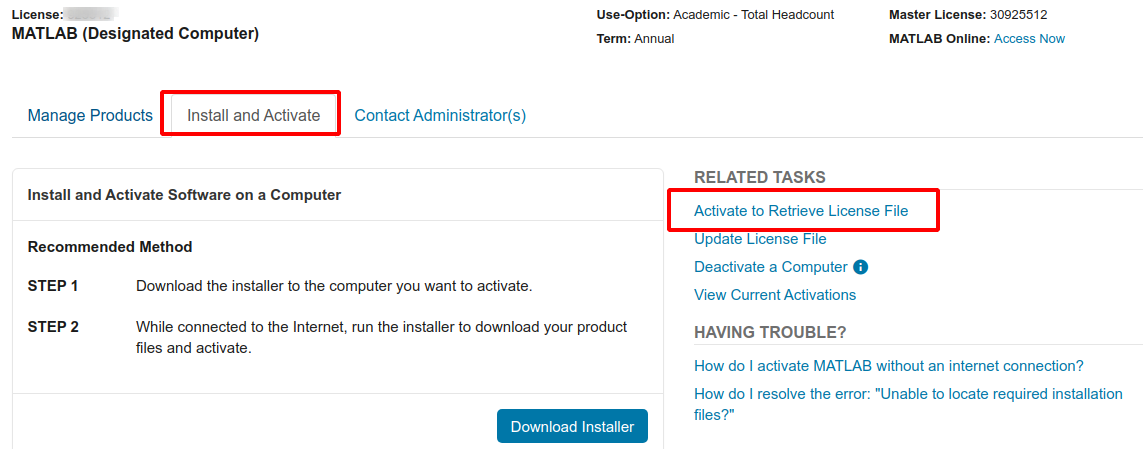
\includegraphics[width=0.7\textwidth]{./pic/license2}
			  \captionsetup{font={small}}
			  \caption{获取许可证步骤二}
			  \label{Fig 获取许可证步骤二}
			\end{figure}

			选择 Activate a Computer 去激活某一台计算机。
			\begin{figure}[H]
			  \centering
			  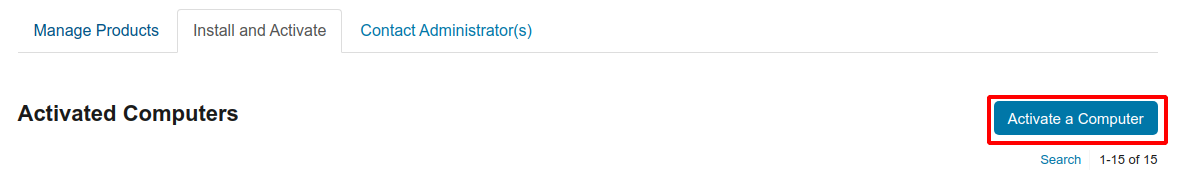
\includegraphics[width=0.7\textwidth]{./pic/license3}
			  \captionsetup{font={small}}
			  \caption{获取许可证步骤三}
			  \label{Fig 获取许可证步骤三}
			\end{figure}

			得到图{\ref{Fig 获取许可证步骤四}}中的图之后
			填写对应的参数,

			\begin{figure}[H]
			  \centering
			  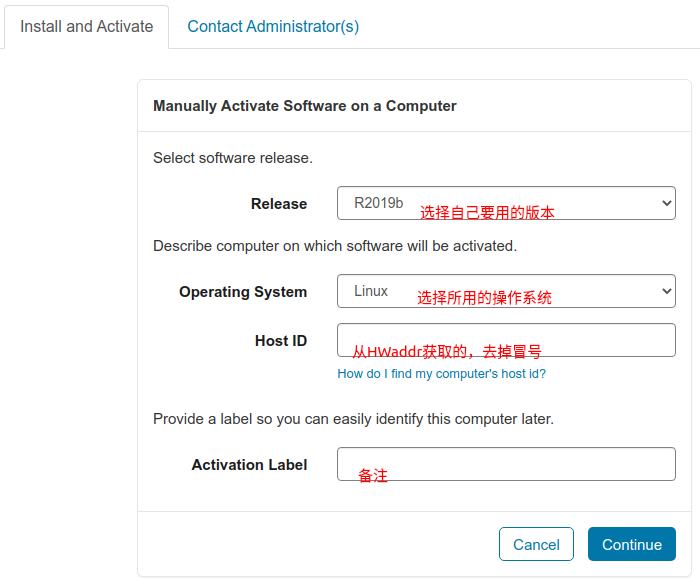
\includegraphics[width=0.5\textwidth]{./pic/license4}
			  \captionsetup{font={small}}
			  \caption{获取许可证步骤四}
			  \label{Fig 获取许可证步骤四}
			\end{figure}

			最终可以得到的许可证 license 文件和安装所需的序列号,
			需要注意的是,
			图片中所显示的序列号并不完整,
			记录时需要查看是否记录完整。

			\begin{figure}[H]
			  \centering
			  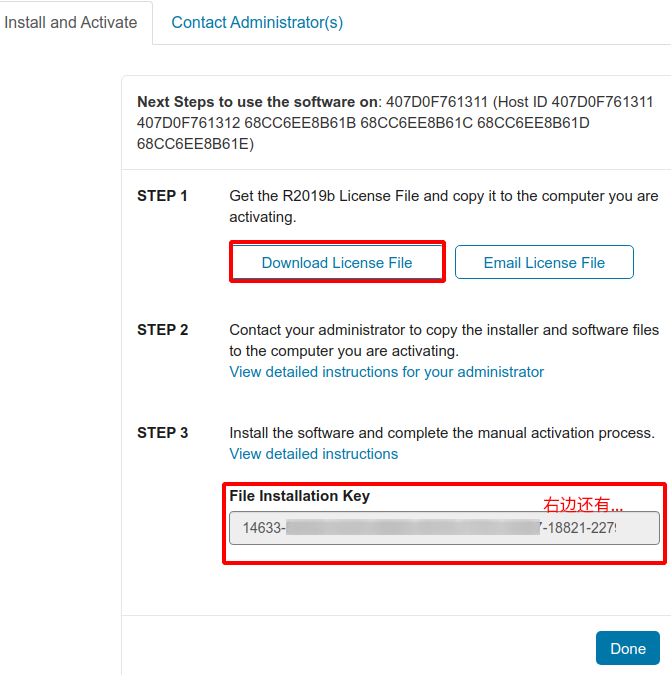
\includegraphics[width=0.5\textwidth]{./pic/license5}
			  \captionsetup{font={small}}
			  \caption{获取许可证步骤五}
			  \label{Fig 获取许可证步骤五}
			\end{figure}
		\end{enumerate}
	\item 加载 iso 文件、配置安装文件
		\begin{enumerate}
		\item 加载 iso 文件

			事先创建一个用于挂载 iso 文件的位置,
			这里采用下面的命令,
			创建了一个名为 cdrom 的文件夹。
			\begin{verbatim}
				$ mkdir /mnt/cdrom
			\end{verbatim}

			回到 iso 文件所在的目录,
			使用下面的命令即可进行挂载 iso 文件:
			\begin{verbatim}
				$ mount -o loop iso.iso /mnt/cdrom
			\end{verbatim}

		\item 配置安装文件

			进入到 /mnt/cdrom/ 目录可以看到一个 installer_input.txt 文件,
			将其复制到 /mnt/cdrom 外, 
			可以是 /mnt 目录,对其进行修改,
			若碰上读写问题,
			可使用 chmod 命令修改权限:
			\begin{verbatim}
				code
			\end{verbatim}

			installer_input.txt 中以两个 \#\# 注释的为说明文字,
			只有一个 \# 注释的表示的为可以设定的参数,
			设定时删除 \# 并添加上对应的参数即可,
			一般只需要修改下面几项即可。

			\begin{itemize}
				\item destinationFolder=自定义路径,例如/usr/local/MATLAB
				\item fileInstallationKey=您自己的FIK
				\item agreeToLicense=yes
				\item outputFile=/tmp/mathworks_install.log
				\item mode=silent (R2020a及以后的MATLAB没有此项配置)
				\item licensePath=许可证文件license.lic的路径
			\end{itemize}


		\end{enumerate}
	\item 静默安装

		安装时终端不能处于 iso 文件挂载的目录中,
		可以退至 /mnt 目录下。
		这样的话可以应用下面的命令调用刚刚配置的 txt 为参数进行安装:
		\begin{verbatim}
			$ cdrom/install -inputFile /mnt/installer_input.txt 
		\end{verbatim}
		
		即可完成安装。

		另一种方式可以不通过读取文件的方式进行安装,
		而是将所需要配置的参数写在命令行进行安装,
		下面的命令只写出一部分,
		剩下的几个参数也是类似的方式进行补全:
		\begin{verbatim}
			$ cdrom/install -agreeToLicense yes -mode silent 剩下省略...
		\end{verbatim}
	\item 激活

		不出意外的话,到这一步就已经完成了 MATLAB 的安装。
		复制 /mnt/cdrom 中的 activate.ini 至 /mnt 中,
		修改其中对应的参数,
		在 MATLAB 安装目录的 bin 文件下,
		可以看到 activate_matlab.sh 文件,
		使用下面的命令来调用 activate.ini 中的参数进行激活即可:
		\begin{verbatim}
			$ ./activate_matlab.sh -propertiesFile /mnt/activate.ini
		\end{verbatim}
		
		若最后即使提示了 Silent activation succeeded。
		但还是说未激活的话,
		可以安装 X11 图形界面,
		通过图形界面进行激活。
	\item 取消挂载 iso 文件

		使用下面的命令即可取消挂载 iso 文件:
		\begin{verbatim}
			$ umount -v /mnt/cdrom
		\end{verbatim}
\end{enumerate}

\subsection{可能碰见的问题}
\label{SubSec 可能碰见的问题}
\begin{enumerate}
\item 提示序列号不正确。

	需要检查序列号是不是填写不全。
	Host ID 是否有误。
\item 打开MATLAB时报错。
	
	MATLAB is selecting SOFTWARE OPENGL rendering.

Fatal Internal Error: Unexpected exception: 'N7mwboost16exception_detail10clone_implINS0_39current_exception_std_exception_wrapperISt13runtime_errorEEEE: Bundle#18 start failed: libXt.so.6: cannot open shared object file: No such file or directory' in createMVMAndCallParser phase 'Creating local MVM'

这是缺少组件 libxt6 ,可在终端中执行下面命令安装组件:
\begin{verbatim}
	$ sudo apt-get install libxt6
\end{verbatim}
\end{enumerate}

\section{MATLAB客服给的方法}
\label{Sec MATLAB客服给的方法}
下面是通过邮件询问客服得到的安装方法的原文。

在安装MATLAB之前,请首先检查要安装的设备是否满足安装要求。您可以从以下的网页中查到相关的详细信息:

\href{https://www.mathworks.com/support/sysreq/previous_releases.html}{https://www.mathworks.com/support/sysreq/previous_releases.html}

1.    准备离线安装文件 ( 已有U盘安装文件的请跳过此步 )

MATLAB.iso镜像文件包含了所有的安装包,许可证管理员也可以在Mathworks网站进行下载。

a)    请打开下面的产品下载网页:

\href{https://www.mathworks.com/downloads/web_downloads/select_release}{https://www.mathworks.com/downloads/web_downloads/select_release}

b)    选择需要安装的产品版本(目前没有提供R2008a及之前版本的ISO文件下载)

c)    点击例如“获取R20XXx ISO映像”的链接进行下载(在页面下方的“相关链接”里,不是特别醒目)


详细的下载操作步骤请参照以下链接:

\href{https://www.mathworks.com/matlabcentral/answers/402492}{https://www.mathworks.com/matlabcentral/answers/402492} 

2.    离线激活MATLAB

激活操作需要获取离线安装电脑的Host ID,激活操作完成后会生成离线安装时需要的许可证文件(License File),并获取到相应的安装密钥(File Installation Key, FIK)。

如何获取安装电脑的Host ID请参照以下链接:

\href{http://www.mathworks.com/matlabcentral/answers/131749}{http://www.mathworks.com/matlabcentral/answers/131749} 

如何进行MATLAB及其他产品的激活请参照以下链接:

\href{http://www.mathworks.com/matlabcentral/answers/309607}{http://www.mathworks.com/matlabcentral/answers/309607}

3.    编辑安装包文件内的installer_input.txt文件的相关项目,为静默安装做准备

\begin{itemize}
	\item destinationFolder=自定义路径,例如/usr/local/MATLAB
	\item fileInstallationKey=您自己的FIK
	\item agreeToLicense=yes
	\item outputFile=/tmp/mathworks_install.log
	\item mode=silent (R2020a及以后的MATLAB没有此项配置)
	\item licensePath=许可证文件license.lic的路径
\end{itemize}

4.    将安装相关的文件夹授予可读写权限

sudo chmod 777 -R 安装包文件路径(例如/home/a/matlab) //把安装源完全授权

sudo chmod 777 -R /usr/local/MATLAB //把安装目标路径完全授权

5.    运行 sudo ./install -inputFile 跟installer_input.txt文件的绝对路径

//例如sudo ./install -inputFile /home/a/matlab/installer_input.txt

\section{参考文档}
\label{Sec 参考文档}
在 iso 中有一份 MATLAB 安装教程,
已经放在 ref 目录下,
搜索 silent 关键词可以找到相应的安装方法,
但是没看到有 silent 模式激活的教程。

\section{Latex工程链接}
\label{Sec Latex工程链接}
本Latex工程的Github链接为:

\href{https://github.com/niyilu45/MATLAB_Slient_Install}{https://github.com/niyilu45/MATLAB_Slient_Install}


\end{document}
